\chapter{Outlier/Anomaly Detection}

In this chapter we looked into the topic of outlier detection. The difficulty of this topic with our dataset is that people have been asked to write a digit, ect 5. One could argue that there are no outliers as no faulty generations of digits have been made and people simply have different ways to write a digit. 

Taking the definition : \textit{An outlier is an observation that differs so much from other observations as to arouse suspicion that it was generated by a different mechanism.} it is our hypothesis that we wont find an outlier, as this would mean we would have to find one single digit that distinct it self from the rest and with 60000 digits, this becomes finding a needle in a haystack.

\section{KNN}
We did an experiment with KNN and five neighbours, to show the five digits in each class that had the largest outlier score. We expected to see something we would classify as being odd digits, but still being able to predict the actual class. Evaluation about them being truth outliers cant be done, but the figure speak for it self.   

\begin{figure}[H]
\centering
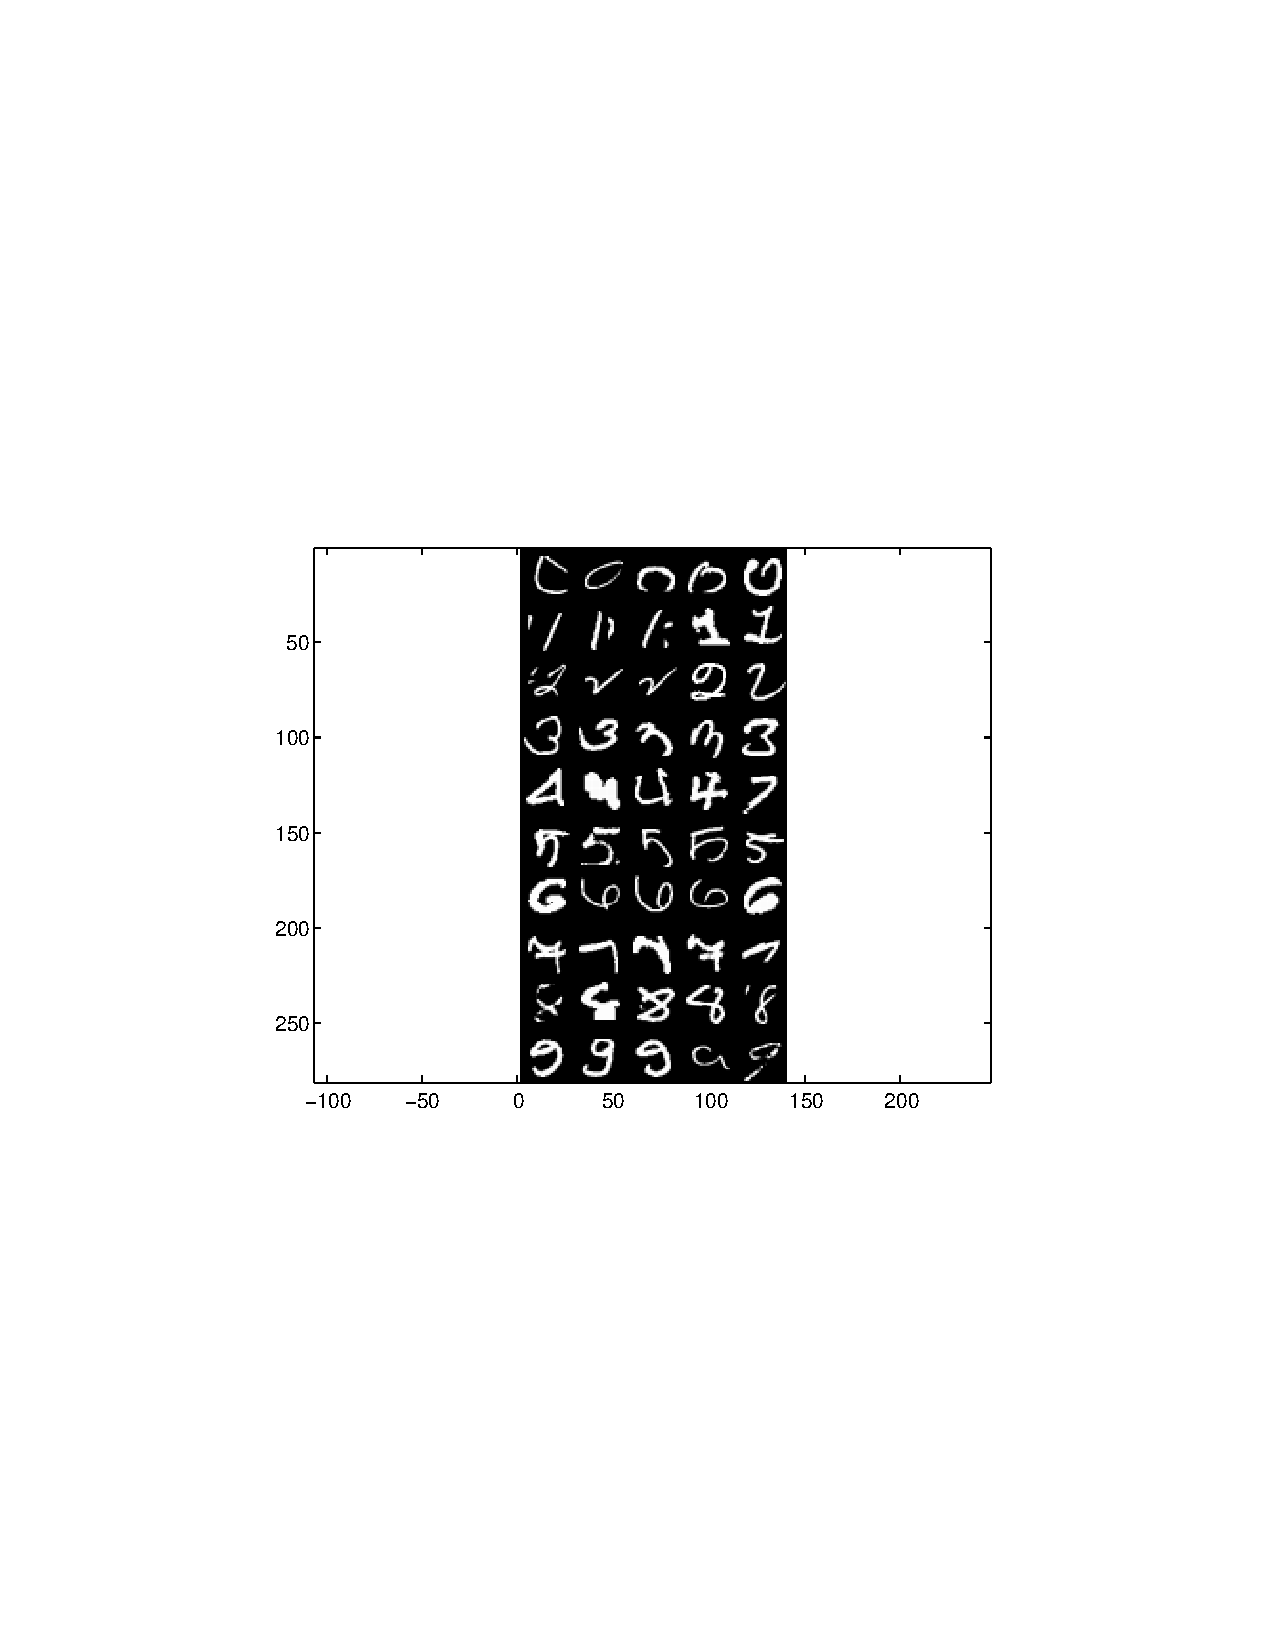
\includegraphics[width=0.6\linewidth]{code/knn_5_outlier}
\caption{The top five outliers from each class found with knn and 5 neighbours.}
\label{fig:outlier_knn}
\end{figure}